
\begin{question}
Please make a frequency table and a frequency histogram from the
following (sorted) continuous data by rounding to the nearest multiple
of 5.

\begin{longtable}[]{@{}rrrr@{}}
\toprule
\endhead
40.8440 & 41.0905 & 42.1430 & 43.2550\tabularnewline
43.5280 & 43.5585 & 44.2030 & 44.6110\tabularnewline
45.4230 & 46.4850 & 46.9060 & 47.1715\tabularnewline
47.1960 & 53.6380 & 58.5405 & 59.0435\tabularnewline
59.9515 & 60.0380 & 61.1855 & 64.4035\tabularnewline
64.5190 & 67.9745 & 69.2705 & 69.5665\tabularnewline
\bottomrule
\end{longtable}
\end{question}

\begin{solution}
Make a frequency table.

\begin{longtable}[]{@{}rr@{}}
\toprule
bin & frequency\tabularnewline
\midrule
\endhead
40 & 3\tabularnewline
45 & 10\tabularnewline
50 & 0\tabularnewline
55 & 1\tabularnewline
60 & 5\tabularnewline
65 & 2\tabularnewline
70 & 3\tabularnewline
\bottomrule
\end{longtable}

Make the histogram.

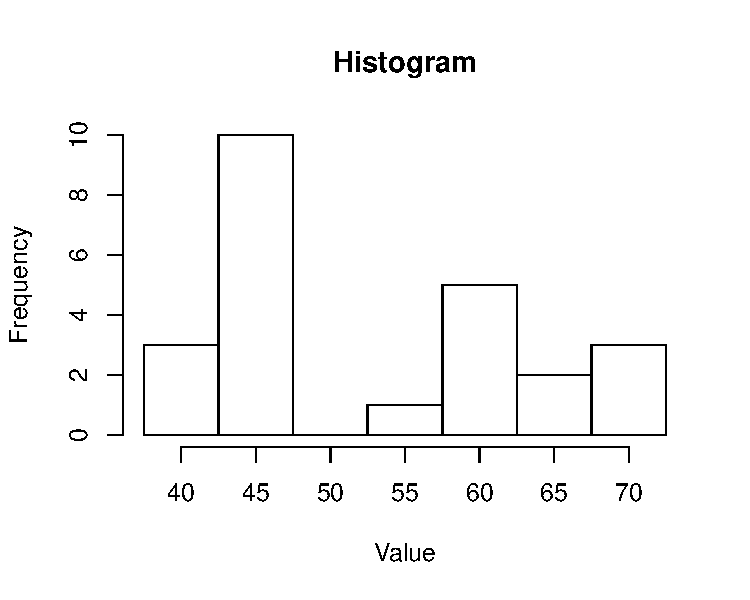
\includegraphics{barchart-1-7.pdf}\\
\end{solution}

